% !TeX root = ../Thesis.tex

%*****************************************
\chapter{Background}\label{ch:relatedwork}
%*****************************************
%%\glsresetall % Resets all acronyms to not used
This chapter provides an understanding of distributed databases, their types, architectures, and data distribution approaches of data sharding and replication. Section \ref{2.1} introduces the concept of distributed databases, differentiates between homogeneous and heterogeneous types, and describes two common architectures, client-server/centralized and peer-to-peer. In section \ref{2.2}, data distribution in distributed databases is discussed in detail, including approaches for data partitioning or fragmentation and replication. Section \ref{shardingDD} discusses the concept of sharding in distributed databases, introducing common five architectural types of sharding. The last section \ref{2.4} of this chapter gives an overview of the related works in distributed databases, specifically in the context of sharding. It discusses the evolution of sharded distributed databases, sharding algorithms, and notable examples of sharded distributed databases in the modern world of big data and blockchain technology.

%***************************************************************************
\section{Distributed Databases}
\label{2.1}
A distributed database is a single logical database comprising of multiple interconnected physical database servers \cite{ramakrishnan2003database, rahimi2010distributed}. It is a collection of multiple, logically interrelated databases that are geographically dispersed but work together to provide an illusion of a single unified system, making the data distribution transparent to end users via a software system, called Distributed Database Management System (DDBMS) \cite{ozsu1999principles}. As the digital revolution ushers into a new era with Big Data in the cloud, the distributed databases aim to accommodate fault tolerance, high availability, reliability, and scalability, addressing the inefficiency and the limitations faced by traditional centralized databases when handling large amount of data \cite{bagui2015database}. \\

\noindent The primary concept of distributed databases is to split up the database and execute queries or transactions in parallel across multiple database servers \cite{ramakrishnan2003database, rahimi2010distributed}. Distributed databases utilize a shared-nothing architecture, in which each database has its own processing unit, local main memory, and storage space, operating independently from the others. In distributed database, data is spread across all the nodes, with each node employing its own Database Management System (DBMS) to manage a specific portion of data and communication between the nodes occurs via a network connection \cite{coronel2016database}. \\

\noindent Distributed databases can be broadly categorized into two types \cite{ozsu1999principles}, described as follows: 
\begin{itemize}
\item[-] \emph{Homogeneous Distributed Databases}: All database nodes in homogeneous distributed databases possess an identical DBMS and adhere to a common global schema. This uniformity simplifies the management of the distributed databases as well as implementation of data distribution strategies. Furthermore, each node is aware of the other nodes’ existence, enabling direct communication and cooperation to process requests from users \cite{silberschatz2011database}.

\item[-] \emph{Heterogeneous Distributed Databases}: In a heterogeneous distributed database, each database node features distinct types of DDMS and operating systems. Heterogeneous distributed databases are more complex, as it requires data integration and management across different systems with varying data models, query languages, and storage structures.
\end{itemize}

\noindent Distributed databases can be further distinguished into two types, based on their architecture, which dictates how the nodes within the system interact and process data. Two common architectures of DDBMS are as follows:

\begin{itemize}
\item[-] \emph{Client-Server / Centralized}: In this architecture, one dedicated coordinator or master database node within the cluster compiles and optimizes requests or queries and manages data across the cluster \cite{silberschatz2011database}. Meanwhile, all other nodes run and process queries in parallel. This approach ensures efficient request handling, although it may introduce a single point of failure if the master database node becomes unavailable.
\item[-] \emph{Peer-to-Peer}: This type of distributed database architecture is conceived as a collection of autonomous databases that interact, establish correspondences, and exchange query and update requests in a peer-to-peer style \cite{10.1145/1374780.1374781}. Data from the local databases can be shared among peers through user requests or queries. Each node in this architecture serves both server and client, resulting in a more resilient system with no single point of failure. However, maintaining data consistency and coordinating updates can be more challenging in a peer-to-peer architecture.
\end{itemize}

\noindent Both architectures have their advantages and drawbacks, and the choice between them depends on system requirements, scalability needs, and the desired level of fault tolerance.

%***************************************************************************

\section{Data Distribution}
\label{2.2}

In distributed databases, the emphasis lies on distributing data across multiple databases. Upon securing the necessary hardware resources and server nodes for deploying distributed databases, it is essential to select an appropriate data distribution model \cite{ costa2015sharding, elmasri2000fundamentals}. Several data distribution techniques, such as fragmentation or partitioning and replication, are employed in distributed databases to manage and store data across multiple nodes. Data distribution encompasses two steps \cite{ramakrishnan2003database, rahimi2010distributed, ozsu1999principles, silberschatz2011database}, which are discussed in the following sections. 


\subsection{Data Partitioning (Data Fragmentation)}

Data partitioning, also known as data fragmentation, divides a single large dataset into multiple segments, called partitions or fragments \cite{mahmud2020survey}. Each partition can be stored at any database node within a computer network. In this process, data is not replicated, i.e., no copies of data are created \cite{venkateswaran2017simplified}. Consequently, data consistency concerns are eliminated, as there is only a single unique instance of data across database nodes. \\

\noindent To prevent data loss, partitions must be created in a way that permits the reconstruction of the original dataset \cite{amiri2019sharding}. Three primary data partitioning strategies \cite{ramakrishnan2003database, rahimi2010distributed, ozsu1999principles, silberschatz2011database, venkateswaran2017simplified, coronel2016database, runceanu2008fragmentation}, which are prevalent in distributed databases are discussed below:

\begin{enumerate}

\item \emph{Horizontal Partitioning:} \\
In horizontal partitioning, a relational table is divided into subsets of one or more rows (tuples) and is also referred to splitting by rows. For non-relational databases, collections of entries or documents are divided into smaller collections comprising constituent entries or documents. For instance, in a key-value store, a large dataset is partitioned into smaller groups of key-value pairs. \\

\noindent Each partition, stored at a distinct node, contains unique data. However, all unique partitions share the same attributes (columns) or fields (sub-entries). In this context, each partition represents the equivalent of a selection operation applied to rows or tuples in relational databases and to entries or documents in non-relational databases. Common horizontal partitioning schemes \cite{runceanu2008fragmentation, elmasri2000fundamentals} are briefly discussed below:

\begin{itemize}

\item [-] \emph{Round-robin:} \\
Round-robin partitioning is the simplest form of horizontal partitioning, where each entry or tuple is sequentially assigned to different partitions. Given n partitions, the i-th entry or tuple of data is allocated to the (i mod n)-th partition. This method is best suitable for evenly distributing data across all partitions without the need for complex analysis and calculations \cite{ozsu1999principles}.

\item [-] \emph{Hash-partitioning:} \\
Hash partitioning uses hash function to fields or attributes of the data that yields a partition number for the placement of the data. This approach ensures a more uniform distribution of data across partitions, regardless of the data's inherent characteristics and patterns \cite{liu1996hash}.

\item [-] \emph{Range-partitioning:} \\
In the range-partitioning approach, range predicates are defined for assigning data to fragments or partitions. This scheme divides data based on value intervals (ranges) of specific attributes or fields. Unlike hash partitioning, which relies on hash functions, range-partitioning requires maintaining the defined ranges in an index structure, such as a B-tree \cite{ozsu1999principles}.

\end{itemize}

\noindent Sharding is a way to scale out a database via horizontal partitioning \cite{runceanu2008fragmentation, rahimi2010distributed}. It enables horizontal scalability (scale-out) is supported by distributing distinct portions of the data across various database servers, a process referred to as sharding. The objective is to direct different requests to individual database nodes, thereby achieving load balancing among the nodes. Concepts and approaches of sharding in distributed databases is further explored in the section \ref{shardingDD}.

\item	\emph{Vertical Partitioning:} \\
Vertical partitioning uses the concept of a projection operator \cite{ozsu1999principles}. In relational database with this partitioning scheme, a relational table with large schema is divided into some more schemas of smaller sizes and is also referred to splitting by columns. For non-relational databases, data is partitioned based on the fields of documents or entries. A common candidate key, also shard key must be present in each partition to guarantee a lossless join between the partitions \cite{navathe1984vertical}.

\item \emph{Hybrid Partitioning:} \\
Both horizontal and vertical partitioning can be nested and combined. The combination of both horizontal and vertical partition together is called hybrid partitioning \cite{6680961}.

\end{enumerate}

\subsection{Data Allocation with Replication}

Deciding on which database server to store data partition is a crucial aspect of data allocation in distributed databases. Data allocation is a critical design issue that significantly impacts the operational efficiency of distributed databases \cite{apers1988data}. Both static and dynamic allocation policies should be carefully considered, and one such data allocation policy is Replication \cite{huang2001fragment, chandra2012dynamic}. 
Replication is also considered a part of data allocation, as it involves assigning data partitions to multiple nodes. Replication entails storing data redundantly at two or more locations. Systems of distributed databases maintain multiple copies of the data due to replication, offering benefits such as increased data availability at numerous locations and parallel handling of data requests \cite{mazilu2010database}.
However, replication also presents certain drawbacks. Data must be updated frequently, and any modifications made to one database server must be reflected at all nodes to prevent inconsistencies \cite{daudpota1998five}. This requirement increases operational and computational overhead. Moreover, concurrency control becomes more complex, as concurrent access must now be monitored across multiple database nodes.

%***************************************************************************
\section{Sharding in Distributed Databases}
\label{shardingDD}
A single machine, or database server, possesses a finite capacity for data storage and processing. When data volume grows too large and surpasses this capacity, the single database node becomes a bottleneck. Data sharding, a common scalability strategy, addresses this limitation by segmenting large dataset into smaller chunks, called shards, and storing them across multiple database nodes \cite{9411547, 9357711, 10.1145/2491245}. Each shard contains unique information, which enables parallel and independent processing across several database nodes. Although operating on distinct database nodes, the shards retain the original database's schema and design. By distributing the workload and reducing the risks associated with a single point of failure, this approach significantly enhances the system's performance, scalability, and resilience. \\

\noindent The implementation of a sharding system in distributed databases requires the initial determination of an appropriate sharding strategy. Database architects must consider the optimal number of shards and the methods for data distribution across multiple servers. Decisions regarding the prioritization of specific requests and the management of bulk data updates and retrieval are vital. A system characterized by frequent data modifications demands a distinct architectural approach for sharding, as opposed to the one that predominantly processes read requests. Additionally, factors such as replication, reliability, and maintenance strategy should be considered. Based on these, sharded databases can be classified into one of the following architectural types: \\

\begin{enumerate}

\item \textit{Range-based Sharding / Dynamic Sharding} \\
This approach involves distributing data based on specified value ranges of shard keys, ensuring that each shard encompasses a continuous segment of the data. For instance, data for users with names starting from A to E could be stored on one database node, while data for users with names between F to J might be stored on another. Range-based sharding, also known as dynamic sharding, is beneficial when data can be readily partitioned based on a distinct key range. It yields good performance, if only a small number of shards are involved to process the request. However, if a request engages multiple shards and requires aggregating the results, the performance would degrade. Nevertheless, the range-scans of data from the databases is efficient \cite{7370983}. \cref{range-shard} illustrates an example of range-based sharding approach. 

\begin{figure}[H]
             \ffigbox{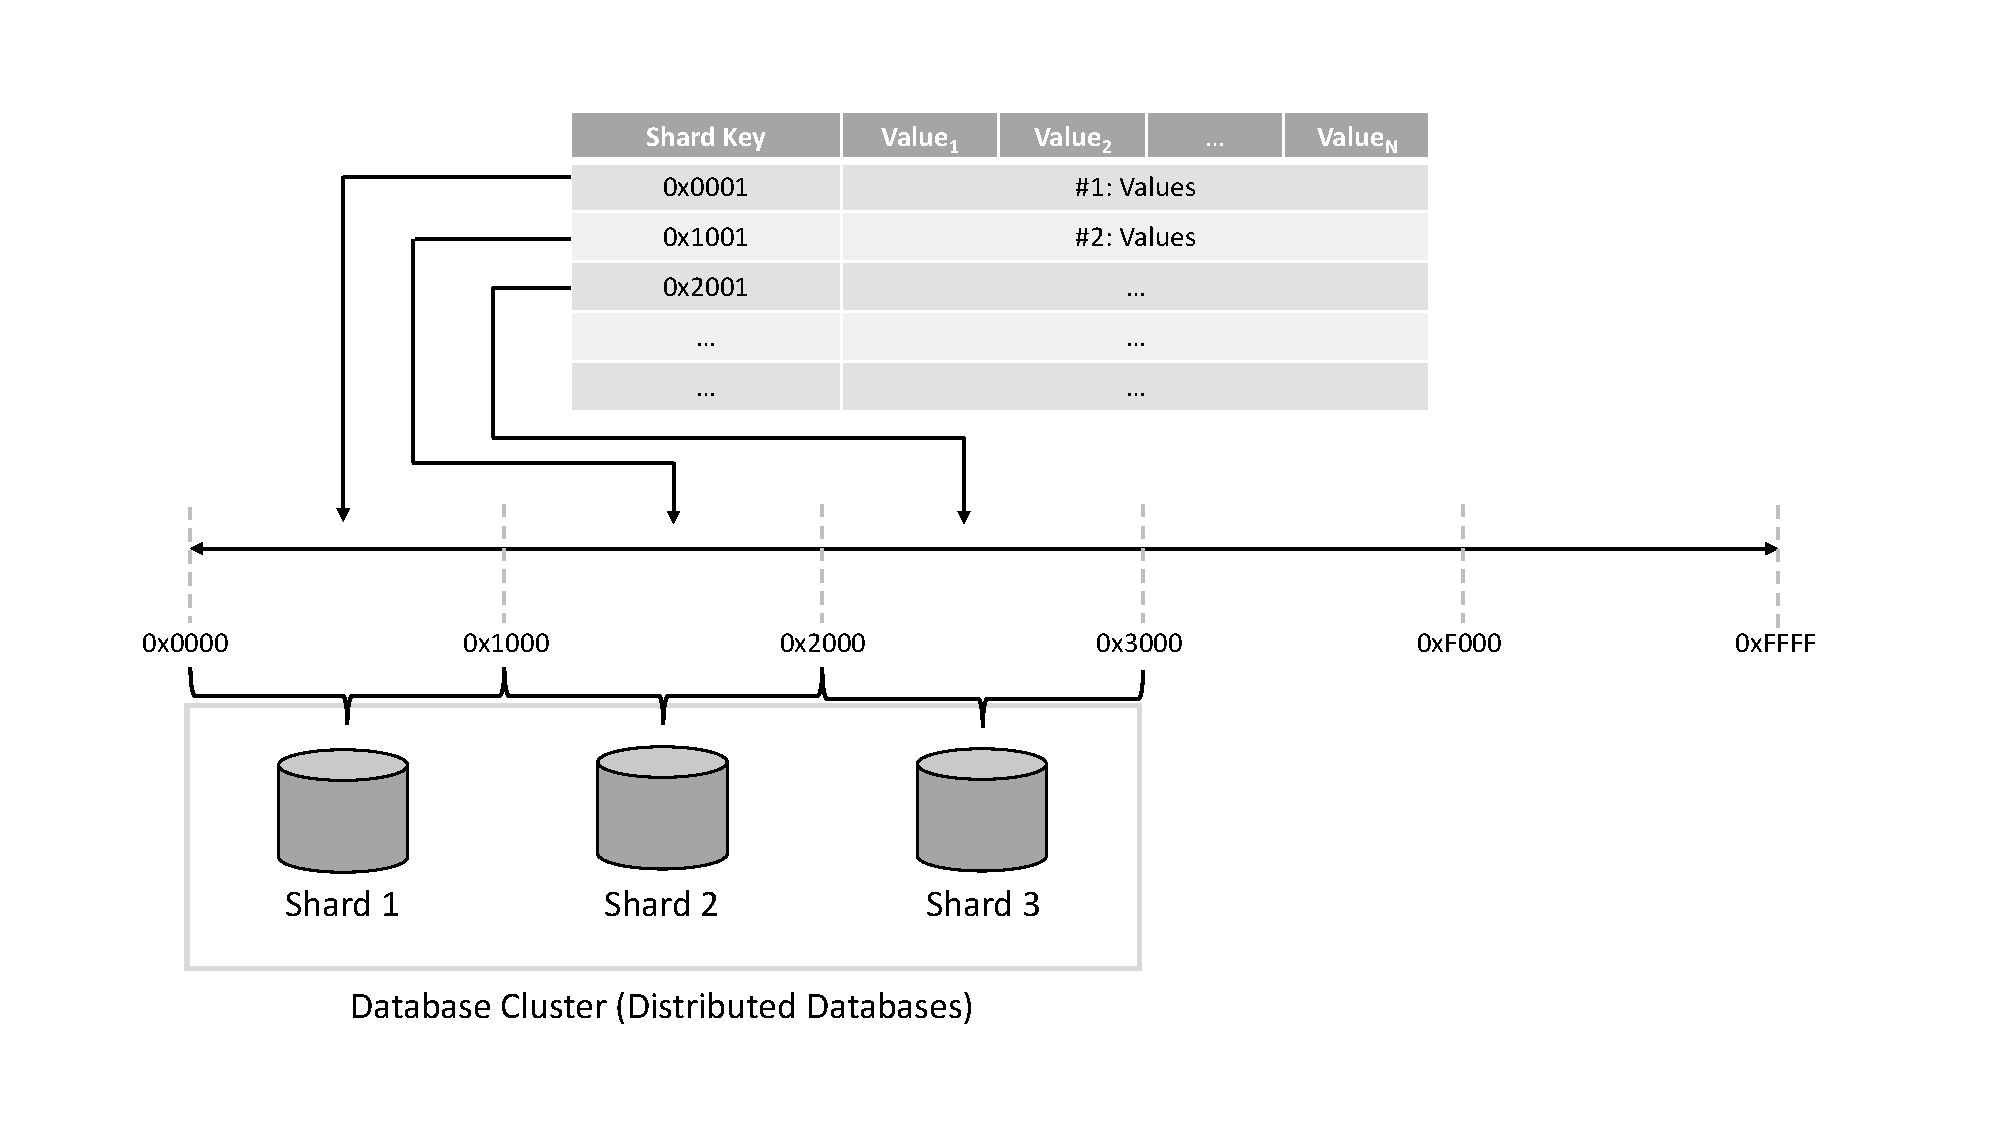
\includegraphics[scale = 0.4]{gfx/design/range_sharding.pdf}}{\caption{Range-based Sharding}\label{range-shard}}
\end{figure}

\noindent This sharding may result in uneven data distribution and overload on a single database node, depending on the data values \cite{Harrison2021, 10.14778/2556549.2556572}. 
In the prior example, the range of values with usernames starting from A to E might have much larger entries than the usernames from F to J. Despite these potential drawbacks, this method is relatively straightforward to implement.

\item \textit{Hash-based Sharding / Algorithmic Sharding} \\
In hash-based sharding, also referred to as algorithmic sharding, a hash function is employed to determine the database node for storing a specific data shard. The hash function accepts a key and generates a hash value (digest), and subsequently determines the data allocation node \cite{costa2015sharding, venkateswaran2017simplified}. \cref{hash-shard} shows an example of hash-based sharding approach. 

\begin{figure}[H]
             \ffigbox{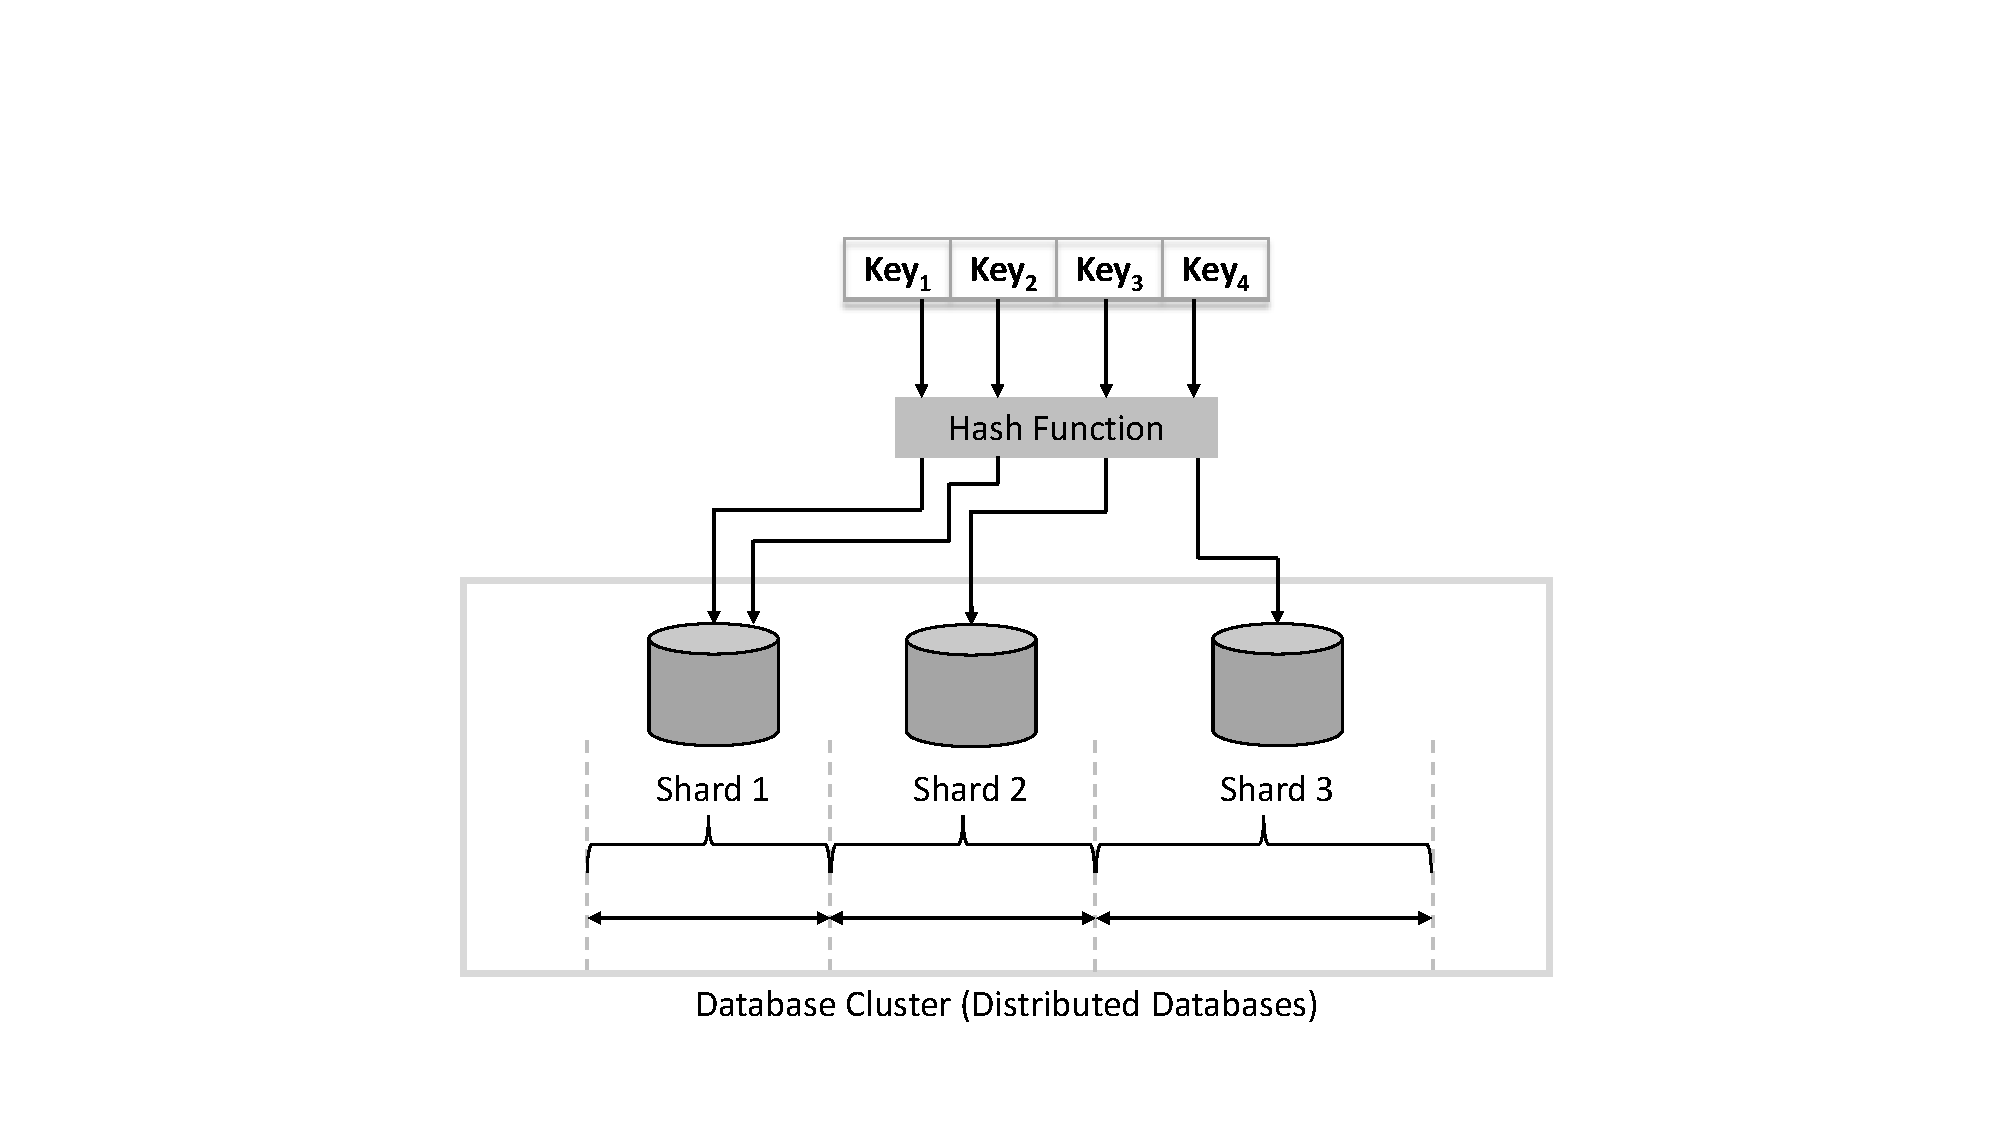
\includegraphics[scale = 0.4]{gfx/design/hash_sharding.pdf}}{\caption{Hash-based Sharding}\label{hash-shard}}
\end{figure}

\noindent Hash-based sharding is favorable when the data lacks a natural key range, and even distribution across sites is crucial. Although this approach ensures uniform data distribution among associated database nodes, it does not shard the data according to any semantically meaningful attributes.

\item \textit{Geo Sharding / Zone-based Sharding} \\
Geo-based sharding or zone-based sharding is a location-aware sharding approach, where data is partitioned based on a user-defined criteria that maps range of data to specific geographical regions and database nodes within those regions. The primary motivation for geo-based sharding is to place data closer in perimeter, both in terms of location and network proximity, to the users and the applications requiring that data \cite{10.1145/2433396.2433424}. Essentially, this method constitutes a range-based sharding, wherein the shard key contains geographic information and the shards themselves are geolocated. For instance, in a dataset feature a "location" field for each entry, performance and system latency can be enhanced by creating a shard for each country or region and storing the corresponding data on that shard \cite{9989965}. \cref{zone-shard} gives an overview of zone-based sharding approach. 

\begin{figure}[H]
             \ffigbox{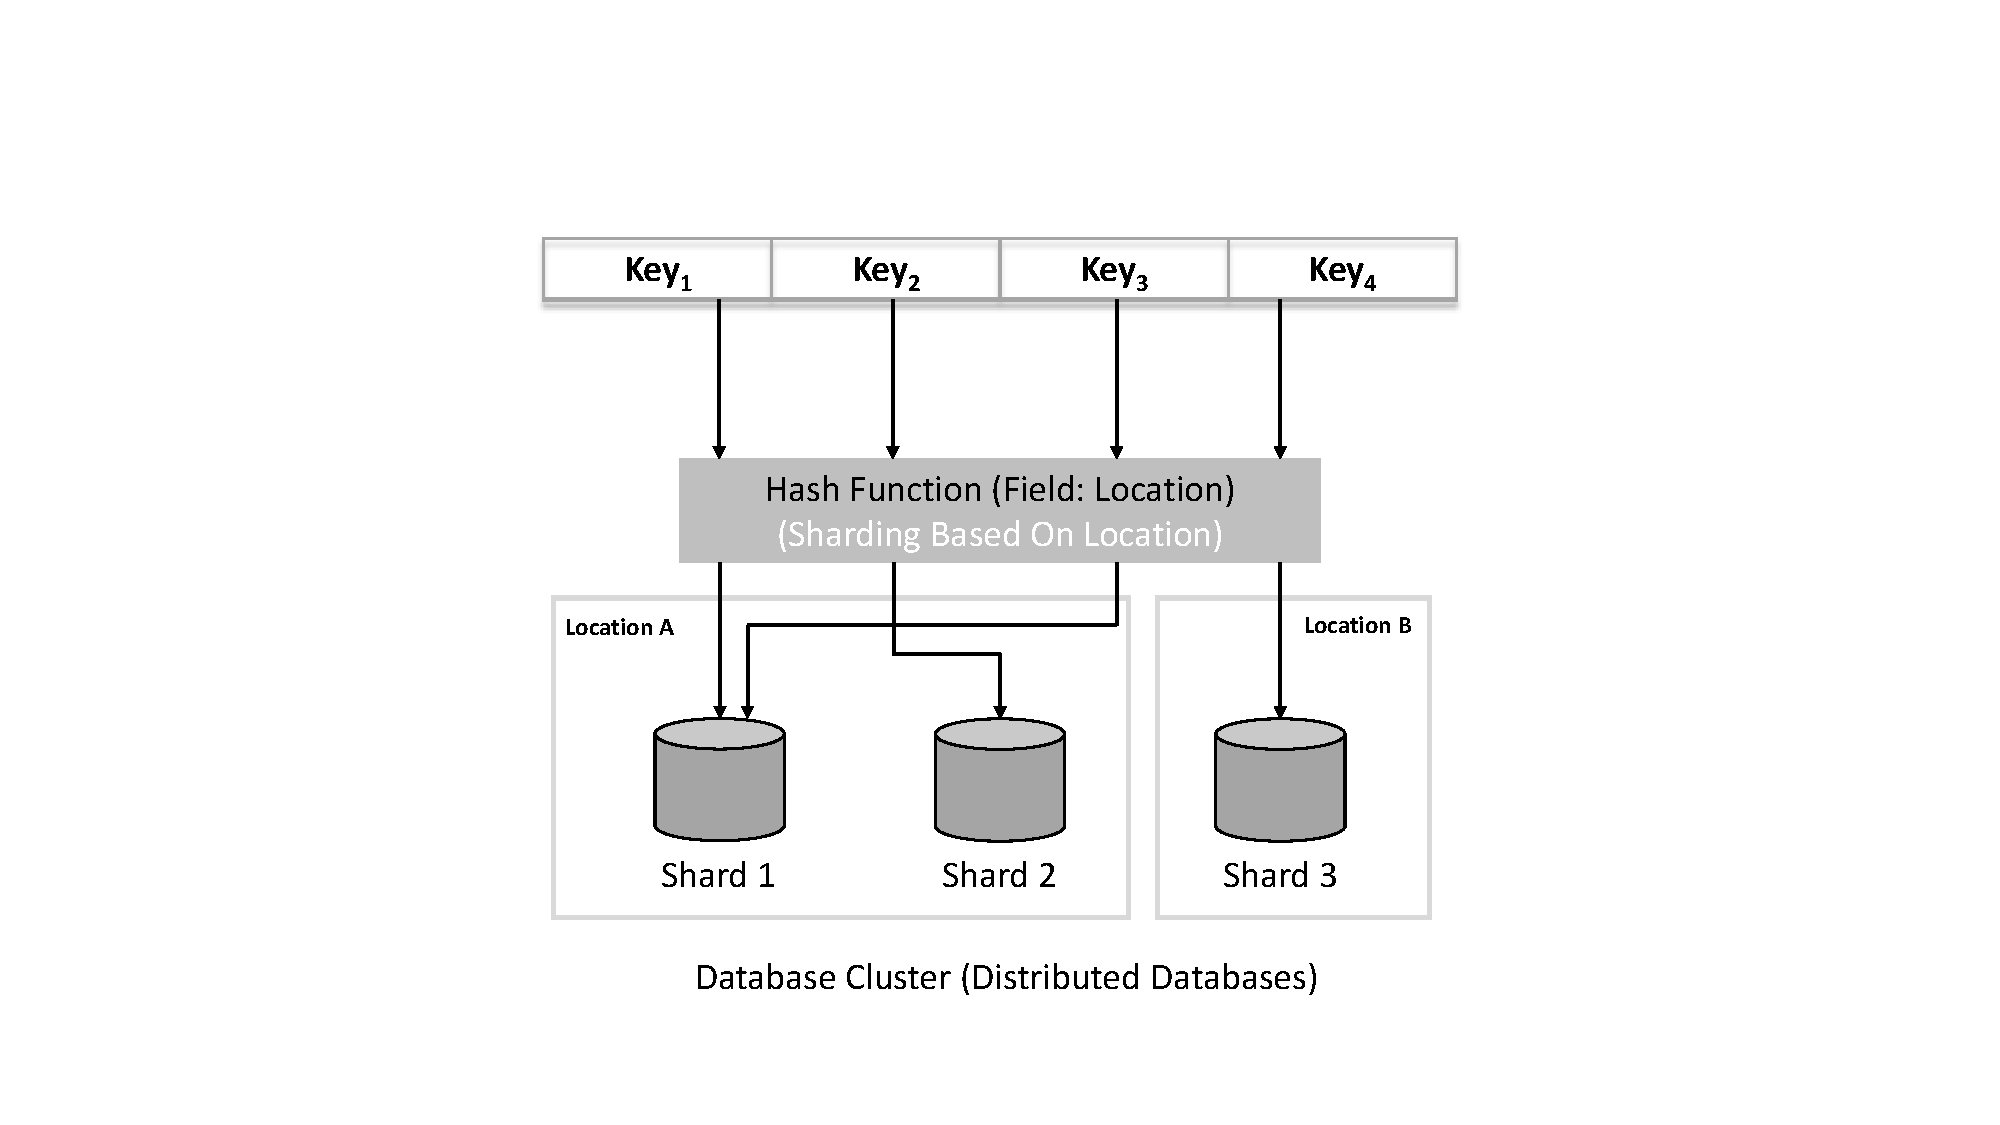
\includegraphics[scale = 0.4]{gfx/design/zone_sharding.pdf}}{\caption{Geo / Zone-based Sharding}\label{zone-shard}}
\end{figure}

\noindent Geo-based sharding proves particularly effective when data access patterns are predominantly based on geography. By partitioning data according to geographic regions or other location-related criteria, this approach offers advantages when it is crucial to store data closer to the users or applications that access it. Nevertheless, geographic-based sharding may lead to imbalanced data distribution across the system, as certain locations may have a higher concentration of users and data flow than others.

\item \textit{Entity-/Relationship-/Directory-based Sharding} \\
This approach utilizes a directory service or lookup table to map data to their corresponding shards, offering flexibility in data distribution and the potential for re-sharding with minimal impact \cite{9357711}. A lookup table holds information about where specific data can be found and, in this context, it uses a shard key to track which shard holds which data. Upon receiving a request for specific data, the appropriate site, i.e., the entry for associated database node in the directory is retrieved based on the shard key. This approach is useful when the number of sites or data distribution is expected to change frequently and when related data must be consolidated within a single physical shard. \cref{directory-shard} illustrates an example of the range-based sharding employed in database systems.

\begin{figure}[H]
             \ffigbox{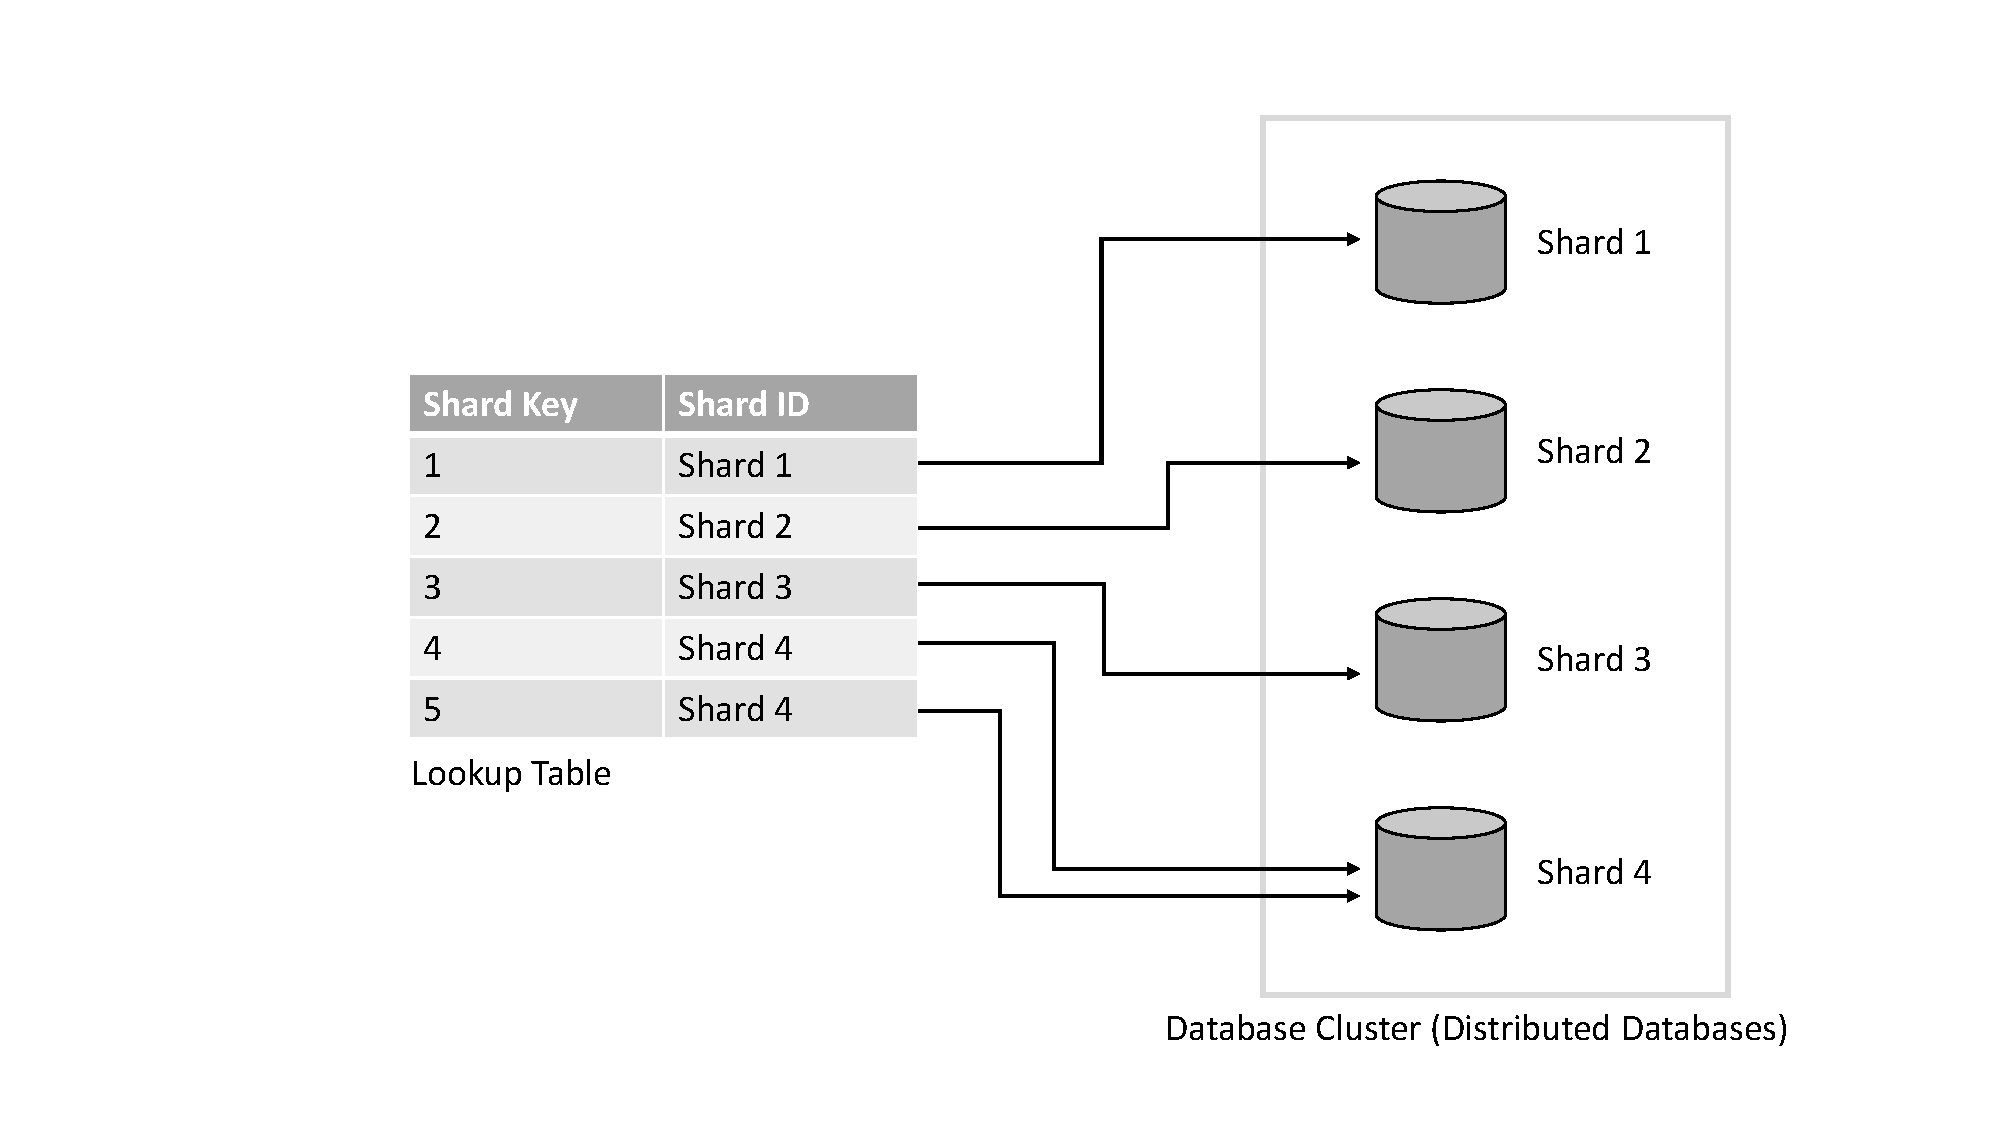
\includegraphics[scale = 0.4]{gfx/design/directory_sharding.pdf}}{\caption{Directory-based Sharding}\label{directory-shard}}
\end{figure}

\item \textit{Multi-level Sharding} \\
This method involves multiple levels of sharding based on data requirements, for instance, data may initially be sharded or partitioned by range, followed by the use of hashing on each key within each range \cite{chen2019sschain}. Multi-level sharding is suitable when scaling the system beyond the capabilities of a single sharding level is essential. 
However, it also introduces added operational complexity and computational overhead. As a result, careful design and planning are essential when implementing this approach.

\end{enumerate}

%***************************************************************************
\section{Related Works}
\label{2.4}
Traditional non-sharded database, typically deployed on a single database server, often becomes a bottleneck for scalability as data and requests increase \cite{schall2015dynamic}. When a single database server is insufficient for handling exceptionally large datasets or extremely high query throughput, sharding, often referred to as partitioning, becomes necessary \cite{ozsu1991distributed}. \\

\noindent Sharding enables distribution of data and query load across multiple database nodes, when processing data on a single database server is no longer feasible. This technique of sharding data and leveraging multiple database servers to process small data partitions or shards in parallel has led to the development of distributed databases \cite{ceri1987distributed}. Numerous works have been carried out on sharding and distributed databases to address the scalability bottleneck and performance issues associated with single database in the face of ever-growing data. New approaches and technologies for better sharding techniques and distributed databases continue to be researched and designed. 
INGRES \cite{stonebraker1976distributed} and SDD-1 \cite{rothnie1980introduction} marked the beginning of distributed databases and introduced the approach of splitting data among multiple database servers, which is a significant step in the evolution of sharded distributed databases. This development implied that distributed databases would provide more write bandwidth and higher availability. Each shard of data would be smaller than the full large dataset, making it faster to backup, recover, and manage. \\

\noindent Sharded databases with shared-nothing architecture were again pioneered in the late 1970s by Teradata, Tandem NonStop SQL, Bubba, and Gamma database systems \cite{stonebraker1986case, KAMAL2016421}. More recently, these concepts have been rediscovered in the era of big data and blockchain technology. Sharded Distributed databases now aim for horizontal scaling or scaling out to address reliability, availability, maintainability, and performance issues, which further solidifies the importance of sharding in modern data management \cite{dewitt1992parallel, mcsherry2015scalability}. \\

\noindent Various sharding algorithms have been proposed in the past, including consistent hashing \cite{karger1997consistent}, range partitioning \cite{curino2010schism}, and directory-based partitioning \cite{mahmud2020survey}.
Recent examples of sharded distributed databases include MongoDB \cite{mongodb}, Amazon DynamoDB \cite{sivasubramanian2012amazon}, Apache Ignite \cite{ignite}, Apache HBase \cite{hbase}, Couchbase \cite{couchbase}, FoundationDB \cite{foundation}, etcd \cite{etcd}, Redis \cite{redis}, Google's Cloud Spanner \cite{spanner}, CockroachDB \cite{cockroach}, etc. These databases employ different sharding strategies and techniques to ensure optimal performance, scalability, and data management in distributed systems. Sharding terminology does indeed vary across many state-of-the-art distributed databases. MongoDB, Elasticsearch \cite{elasticsearch}, and SolrCloud \cite{solrcloud} use the term "shard”, Apache HBase uses "region”, Google’s Bigtable \cite{chang2008bigtable} uses "tablet”, Cassandra \cite{cassandra2014apache} and Riak \cite{klophaus2010riak} use "vnode", and Couchbase uses "vBucket." Despite the differences in terminology, all these terms fundamentally represent blocks or chunks of data derived from a large dataset. \\

\noindent Google's Cloud Spanner \cite{spanner} and Apache Cassandra \cite{cassandra2014apache} are notable examples of sharded distributed databases that have made significant contributions to the field. Both databases have been designed with scalability, high availability, and distributed data management in mind, making them well-suited for handling big data.
Google's Spanner is a globally distributed database that shards data across multiple sets of Paxos state machines \cite{corbett2013spanner}. It offers high availability and geographic locality by sharding data and migrating it across machines to balance the load and respond to failures. Apache Cassandra, inspired by the range sharding of Google's Bigtable and the consistent hash sharding of Amazon's DynamoDB, is a popular distributed database choice for big data management \cite{chebotko2015big}. It ensures zero downtime, linear scalability, and seamless deployment across multiple data centers. Cassandra adopts a linear hash sharding approach, which is a hybrid of range and consistent hash sharding methods. Both Spanner and Cassandra have significantly advanced the field of sharded distributed databases, highlighting how these systems can effectively handle large-scale data management challenges with resilience, scalability, and performance. \\

\noindent Sharding approaches also play a vital role to enhance the performance of search engines, by helping to distribute data and workload across multiple database servers, enabling more efficient parallel processing and faster query response times \cite{DHULAVVAGOL20201626}. The primary goal of search engines is to refine user queries and retrieve only relevant documents from the appropriate shards while disregarding irrelevant data from other shards \cite{mohammad2018dynamic}.
In \cite{elasticShard} different sharding techniques are implemented and evaluated using the Elasticsearch platform, a widely used search and analytics engine. The objective is to develop a mechanism that can handle large-scale data processing and searching operations effectively through efficient sharding techniques. \\

\noindent Sharding is also used for achieving scalable blockchains, as it addresses the inherent limitations of existing blockchain systems, such as low transaction throughput, long confirmation times, and increasing storage requirements \cite{croman2016scaling}. These challenges stem from the fact that every node in a traditional blockchain network stores and processes the entire transaction history, leading to inefficiencies as the network size grows \cite{zamani2018rapidchain}. In blockchain systems, sharding is employed to divide the network into smaller, manageable partitions or shards. Each shard processes a subset of transactions independently, thereby increasing overall throughput and reducing the storage and processing burden on individual nodes. This approach allows for the parallel processing of transactions and enhances the network's scalability. Several new protocols have been developed to use sharding as part of the blockchain consensus protocol to address the scalability challenge of blockchains \cite{sonnino2018chainspace, kokoris2018omniledger, zamani2018rapidchain}.





